\documentclass[11pt, oneside]{article}
\usepackage[letterpaper, margin=2cm]{geometry}
\usepackage{AERE546}
\usepackage{xspace}

\begin{document}
\noindent \textbf{\Large{Caleb Logemann \\
AER E 546 Fluid Mechanics and Heat Transfer I \\
Homework 3
}}

%\lstinputlisting[language=MATLAB]{H01_23.m}
\begin{enumerate}
  \item % #1 Done
    A slab of metal is initially at uniform temperature.
    One end is suddenly raised to a high temperature, while the other end is kept cool.
    Compute the penetration of heat into the slab as a function of time.
    In dimensional form the temperature diffusion equation, initial and boundary values are
    \[
      \pd{T^*}{t_*} = \kappa \pd[2]{T^*}{x_*} \qquad T^*(x,0) = 0 \qquad T^*(0, t) = 0, T^*(L, t) = T_w.
    \]
    Non-dimensionalize temperature by $T_w$ and length by $L$ and time by $L^2/\kappa$.
    Integrate by Euler Explicit, up to a non-dimensional time of $0.3$.
    Use $N_x = 121$ grid points in $x$.
    Let $\Delta t = \alpha \Delta x^2$.
    Try a value of $\alpha > 0.5$.
    What happens?
    Why?
    How small must $\alpha$ be to obtain an accurate solution?
    Provide a single figure with line plots of the solution at time intervals of 0.04.
    Note that the computational time-step will be smaller than 0.04.
    The bulk heat transfer coefficient is defined as
    \[
      h_T = \frac{Q}{T(1) - T(0)}
    \]
    where $T = \eval{\pd{T}{x}}{x = 1}{}$ is the heat flux into the slab.
    Plot $h_T$ as a function of time for $t > 0.01$.

    First I will nondimensionalize this equation by doing the following substitutions.
    \begin{gather}
      T^* = T_w T \\
      x^* = L x \\
      t_* = \frac{L^2}{\kappa} t
    \end{gather}
    Now the differential equation can be simplified as follows.
    \begin{gather}
      \pd{T^*}{t_*} = \kappa \pd[2]{T^*}{x_*} \\
      T_w \pd{T}{t_*} = \kappa T_w \pd[2]{T}{x_*} \\
      \frac{T_w \kappa}{L^2} \pd{T}{t} = \frac{\kappa T_w}{L^2} \pd[2]{T}{x} \\
      \pd{T}{t} = \pd[2]{T}{x}
    \end{gather}
    The initial and boundary conditions are given as
    \[
      T(x, 0) = 0 \qquad T(0, t) = 0 \qquad T(1, t) = T_2
    \]

    Now this non-dimensionalized PDE can be descretized in space as follows
    \[
      \dot{T}_j = \frac{T_{j+1} - 2T_j + T_{j-1}}{\Delta x^2}
    \]
    If the time derivative is solved with Euler Explicit then the update formula
    becomes
    \[
      T^{n+1}_j = T^n_{j} + \frac{\Delta t}{\Delta x^2}\p{T_{j+1} - 2T_j + T_{j-1}}
    \]

    The following function implements this Euler Explicit update.
    \lstinputlisting[language=MATLAB]{forwardEuler.m}
    The following script now uses the forwardEuler function to compute a
    solution to the non-dimensional problem.
    \lstinputlisting[language=MATLAB, lastline=46]{H03.m}
    The script outputs the following two images.
    \begin{center}
      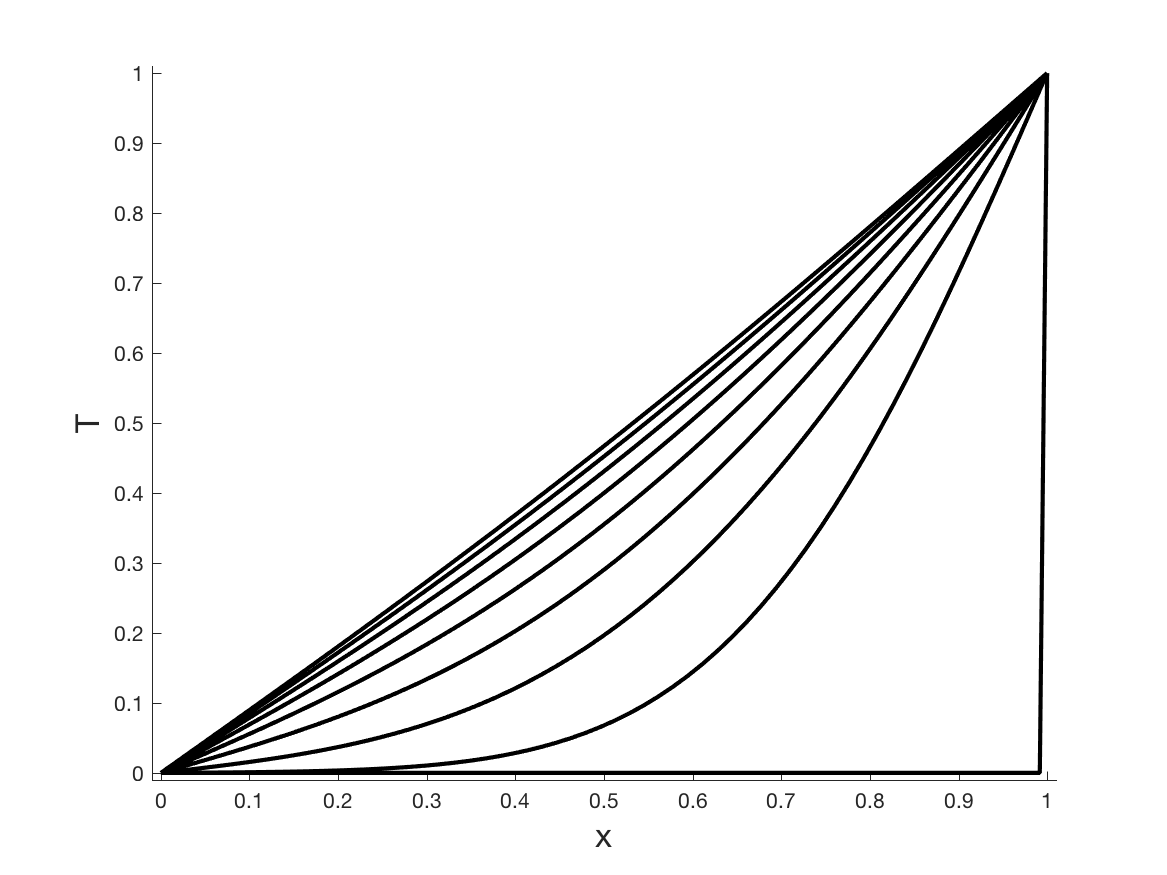
\includegraphics[scale=0.5]{Figures/03_01.png}
      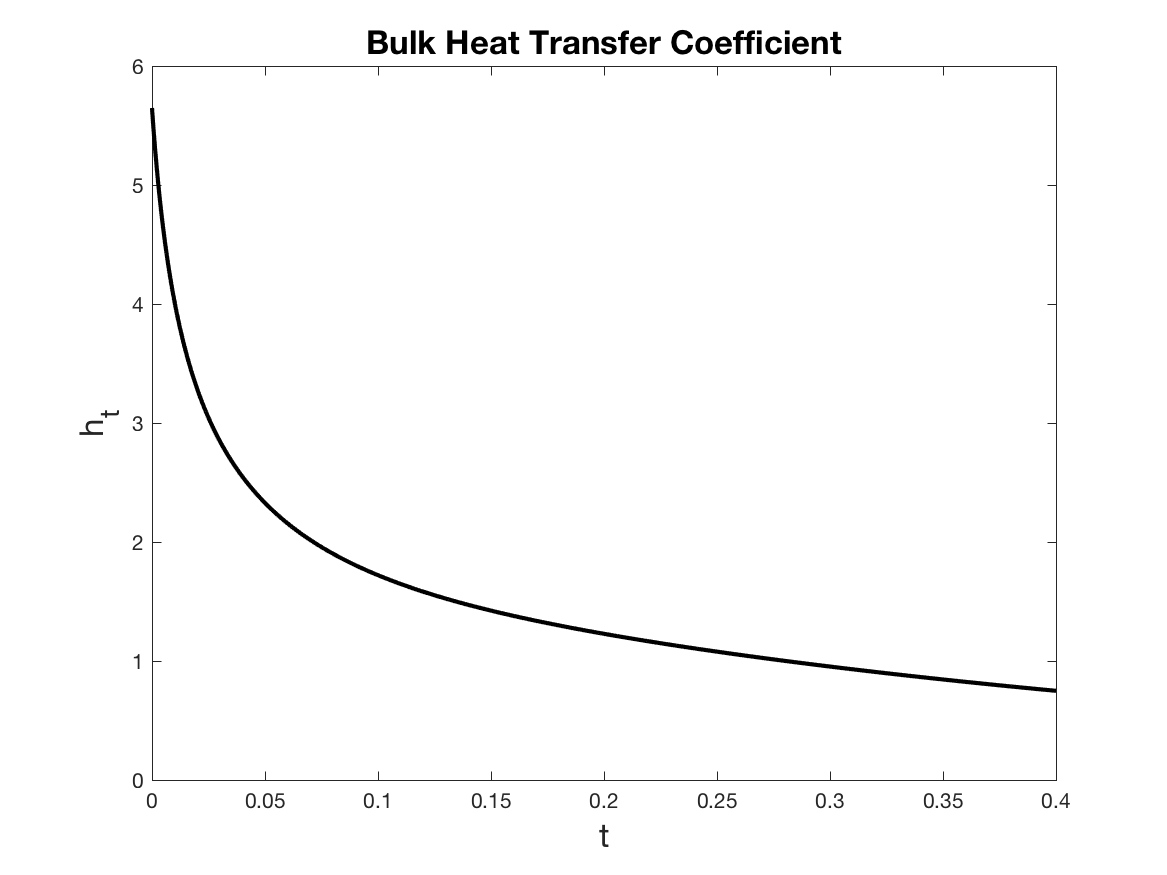
\includegraphics[scale=0.5]{Figures/03_02.png}
    \end{center}

  \item % #2 Done
    A slab is heated by shining a laser on it.
    The laser is shut off and the heat diffuses throughout the slab.
    Its ends are insulated.
    This is modeled as the non-dimensional problem: solve
    \[
      \pd{T}{x} = \pd*{\kappa \pd{T}{x}}{x}
    \]
    in the interval $0 \le x \le 1$, with the initial condition
    \[
      T(x, 0) = \frac{e^{-\p{x - 0.5}^2/\sigma^2}}{\sigma \sqrt{\pi}}, \quad \sigma = 0.1
    \]
    The slab length is normalized to unity and $\sigma$ characterizes the
    region heated by the laser.
    Consider a material with variable diffusivity.
    Let
    \[
      \kappa = 0.1 + 2.0 e^{-5x}
    \]
    The no-flux boundary condition
    \[
      \pd{T}{x}(0, t) = 0 = \pd{T}{x}(1, t)
    \]
    is applied at the insulated ends.
    Use second order Runge-Kutta.
    Solve with about $N_x = 250$ grid points in $x$.
    Choose a small time-step to obtain an accurate solution.
    Integrate up to a non-dimensional time of 0.05.
    Provide a single plot containing the initial condition and curves showing
    the solution $T(x)$ at time intervals of 0.01.
    Plot $\dintt{0}{1}{T(x)}{x}$ versus time.
    What should the value of the integral be?

    Since the slab has a variable diffusivity, this problem can not be
    discretized in space the same way as before.
    I chose to rewrite the problem as
    \[
      \pd{T}{t} = \kappa'(x) \pd{T}{x} + \kappa(x) \pd[2]{T}{x}
    \]
    I then use the standard central finite difference approximations for the
    first and second space derivatives.
    This results in the following set of ODEs
    \[
      \dot{T}_j = \kappa'(x_j) \frac{T_{j+1} - T_{j-1}}{2\Delta x} + \kappa(x_j) \frac{T_{j+1} - 2T_j + T_{j-1}}{\Delta x^2}
    \]
    The exact value of the derivative of $\kappa$ can be used.
    \[
      \kappa'(x) = -10.0 e^{-5x}
    \]
    This system of ODEs can now be solved using RK2.
    The following function implements RK2.
    \lstinputlisting[language=MATLAB]{rk2.m}
    The following script now uses this function to solve the system of ODEs
    given earlier.
    \lstinputlisting[language=MATLAB, firstline=48 ,lastline=95]{H03.m}
    The script outputs the following two images.
    The first image shows the temerature distribution over time.
    The second image shows the integral of the temperature over time.
    Note that since both ends of the slab are insulated no energy should be
    leaving the slab, so this plot should be constant at 1.
    This is not exactly true, but the total integral only decreases by about
    $0.000008$, so energy is almost exactly conserved.
    It is also good to note that this is a decrease in energy, no extra heat is
    being generated.
    \begin{center}
      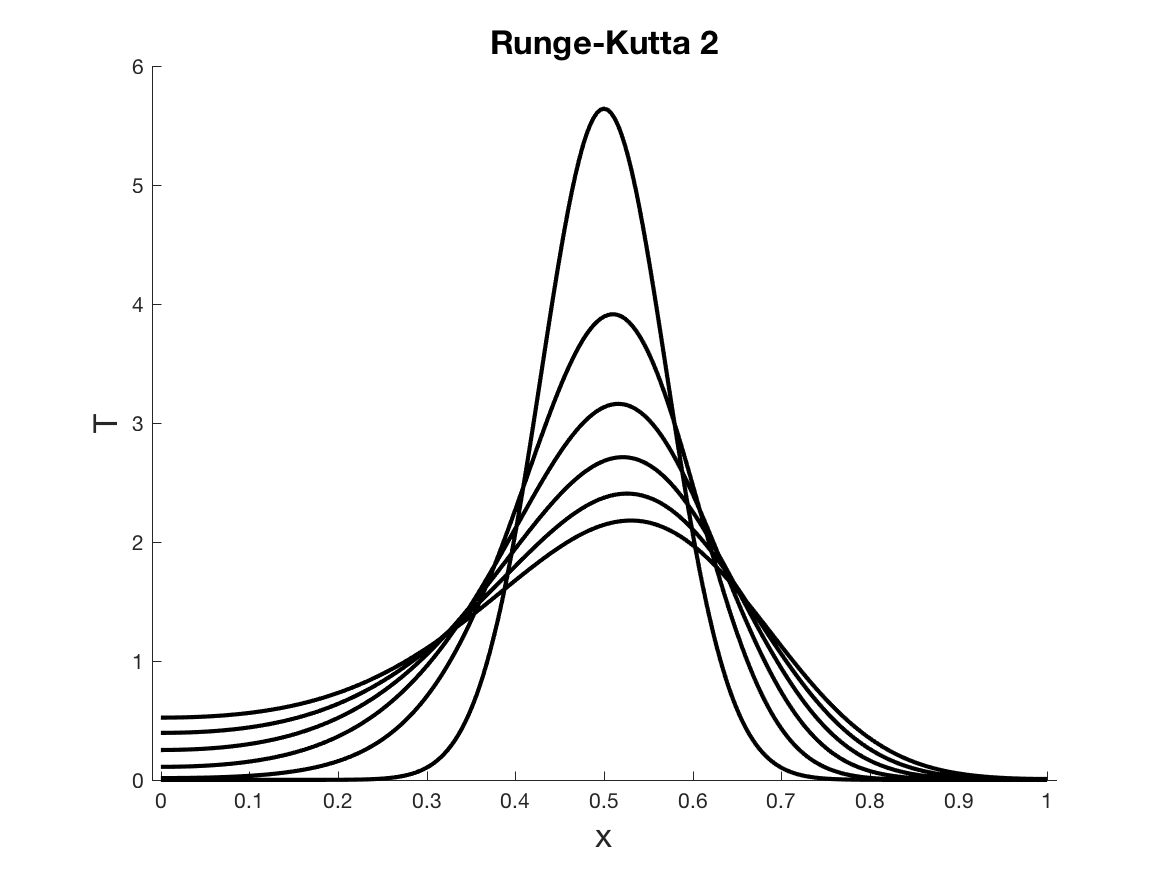
\includegraphics[scale=0.5]{Figures/03_03.png}
      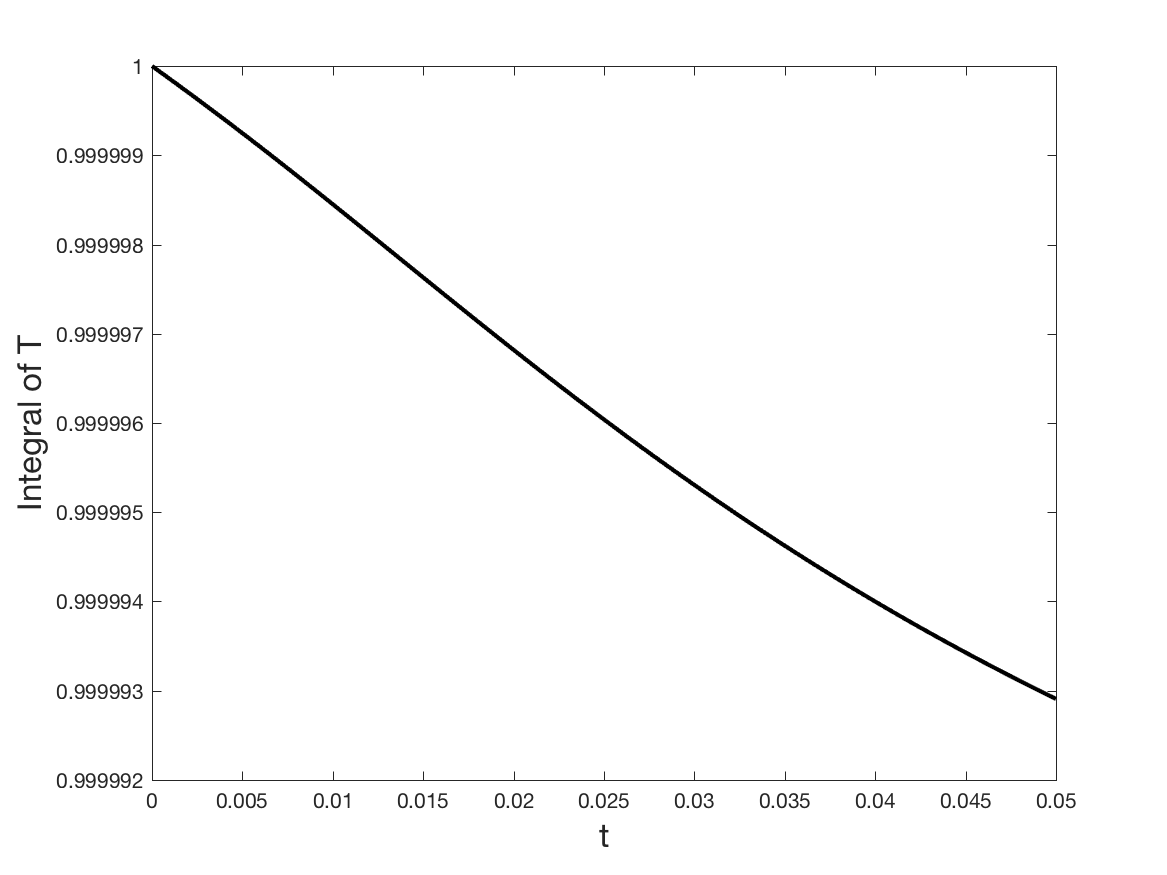
\includegraphics[scale=0.5]{Figures/03_04.png}
    \end{center}

  \item % #3 Done
    Now consider the case where one end of the slab is insulated and the other
    is held at constant temperature:
    \[
      \pd{T}{x}(0) = 0 \quad T(1) = 1
    \]
    solve the constant diffusivity, diffusion equation as in the first problem,
    but use Crank-Nicholson.
    \begin{enumerate}
      \item[(a)] % Done
        Set $\Delta t = \alpha \Delta x^2$.
        Try a couple of relatively large value of $\alpha$ and see whether your
        calculation converges, or blows up (should it?).

        Using some large values of $\alpha$, like $\alpha = 10$, I see that the
        solution does converge.
        It doesn't blow up, I do see some strange behavior in the bulk heat
        transfer coefficient at the beginning of the simulation, but the
        numerical solution still converges to the correct solution.
        This is because the Crank-Nicholson method is absolutely stable for any
        time-step.

      \item[(b)] % Done
        Provide a single figure with plots of $T(x)$ at intervalue of $0.04$ up to $t = 0.4$.
        Explain why your solution makes sense.
        The bulk heat transfer coefficient is defined as
        \[
          h_T = \frac{Q}{T(1) - T(0)}
        \]
        where $T = \eval{\pd{T}{x}}{x = 1}{}$ is the heat flux into the slab.
        Plot $h_T$ as a function of time for $t > 0.01$.

        The following function implements the Crank-Nicholson method.
        \lstinputlisting[language=MATLAB]{crankNicholson.m}

        The following script now uses this Crank-Nicholson function to solve
        the heat diffusion equation given previously.
        \lstinputlisting[language=MATLAB, firstline=97]{H03.m}
        The following two images are produced.
        The first image shows the temperature distribution over time.
        This solution makes sense because as more heat flows in from the right
        side and is unable to escape the insulated left side the solution
        approaches a steady state of constant temperature.
        The bulk heat transfer plot shows that a lot of heat diffuses in to the
        slab at first, but then slows as the temperature gradient decreases.
        \begin{center}
          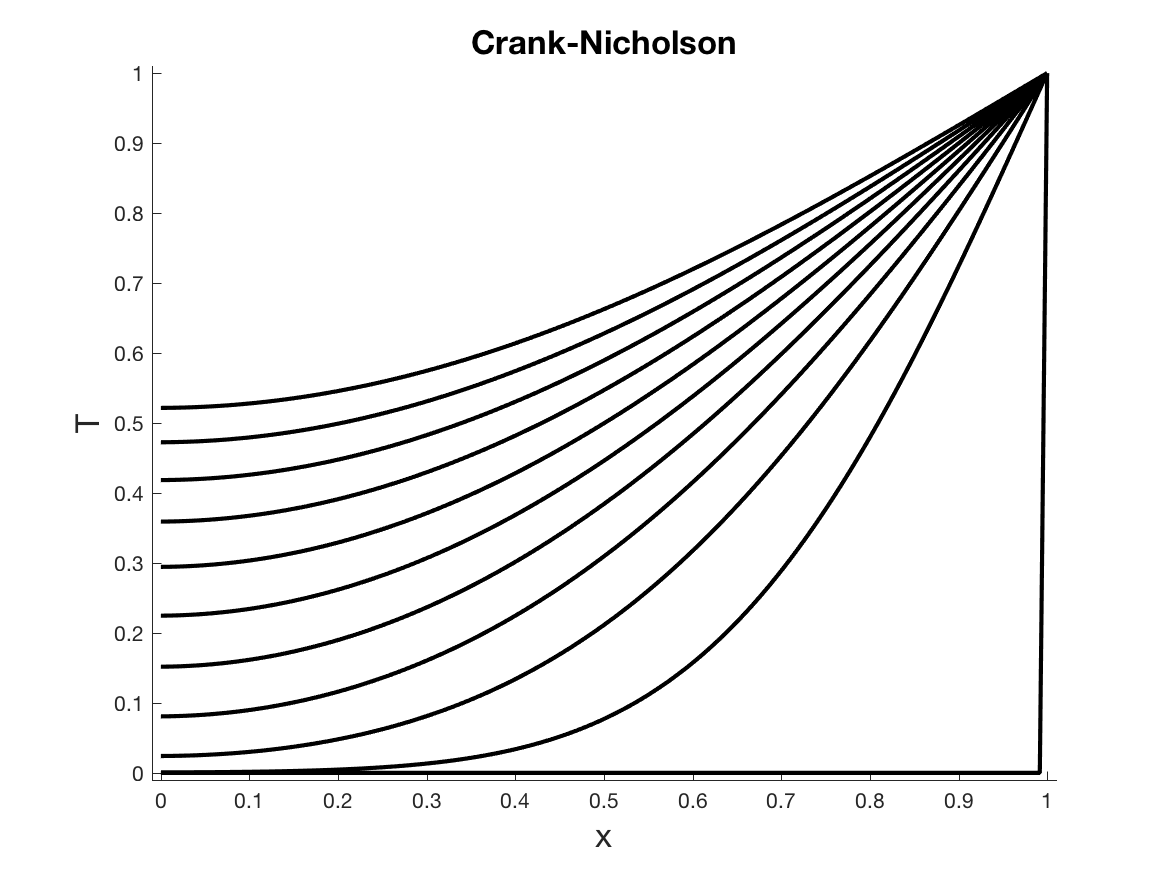
\includegraphics[scale=0.5]{Figures/03_05.png}
          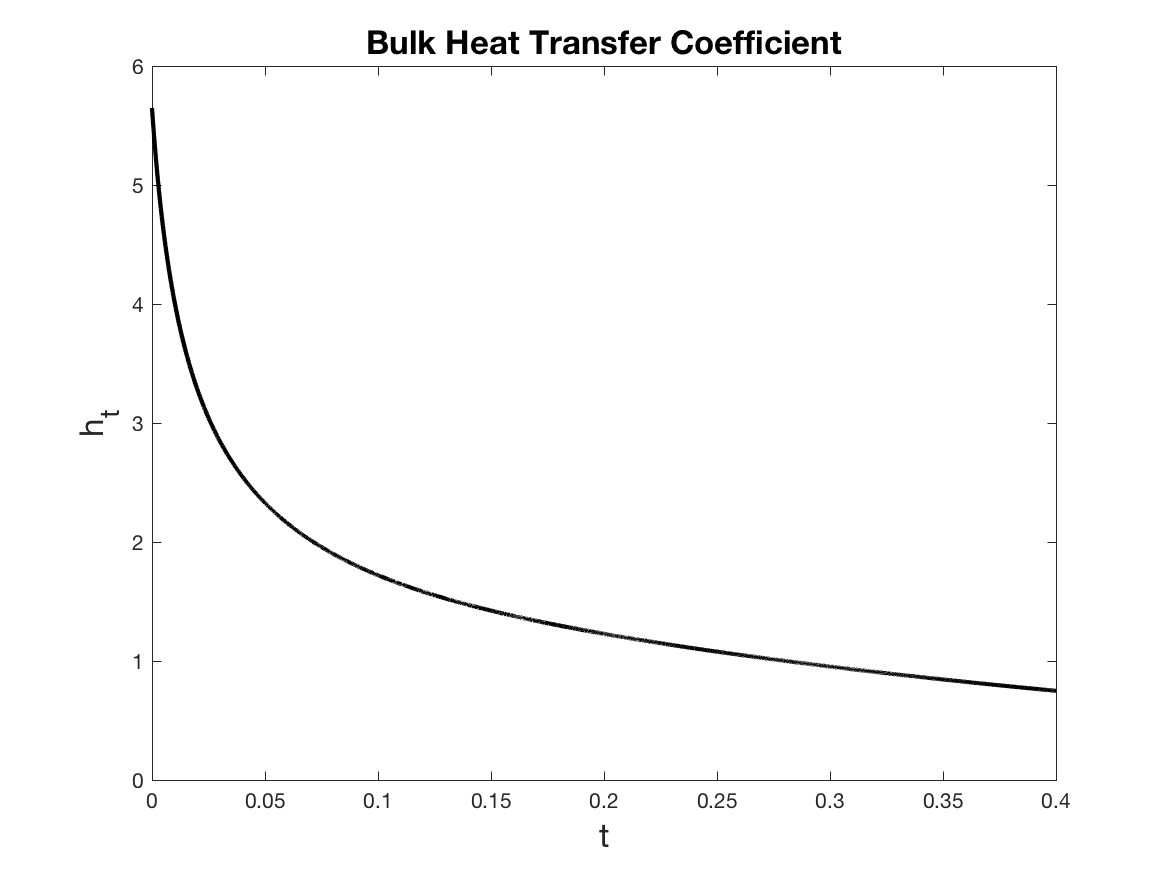
\includegraphics[scale=0.5]{Figures/03_06.png}
        \end{center}
    \end{enumerate}

  \item % #4 Done
    \begin{enumerate}
      \item[(a)] % Done
        Is the scheme
        \[
          U_i^{n+1} = U_i^n - \frac{C}{2} \p{U_{i+1}^n - U_{i-1}^n}
        \]
        stable, conditionally stable or absolutely unstable?
        C is a constant.

        In order to perform a Von Neumann Stability, each term needs to be
        replaced with an error approximation.
        Let $\epsilon^n_i$ be the error at $x_i$ at time $t_n$.
        Approximating this error with white noise implies that
        $\epsilon^n_i = e^{\alpha t} e^{i k_m x_i}$.
        Now $\abs{e^{\alpha \Delta t}}$ represent the growth of the error from
        one time step to another.
        If $\abs{e^{\alpha \Delta t}} \le 1$, then the error decreases over time
        and the method is stable.
        \begin{gather}
          \epsilon^{n+1}_i = \epsilon_i^n - \frac{C}{2} \p{\epsilon_{i+1}^n - \epsilon_{i-1}^n} \\
          e^{\alpha (t + \Delta t)} e^{i k_m x_i} = e^{\alpha t} e^{i k_m x_i} - \frac{C}{2} \p{e^{\alpha t} e^{i k_m (x_i + \Delta x)} - e^{\alpha t} e^{i k_m (x_i - \Delta x)}} \\
          e^{\alpha \Delta t} = 1 - \frac{C}{2} \p{e^{i k_m \Delta x} -  e^{-i k_m \Delta x}} \\
          \abs{e^{\alpha \Delta t}} = \abs{1 - C \p{i \sin{k_m \Delta x}}} \\
          \abs{e^{\alpha \Delta t}} = \sqrt{1 + C^2 \sin[2]{k_m \Delta x}} \\
        \end{gather}
        Note that this is always greater than one because $C^2 \sin[2]{k_m \Delta x} > 0$.
        This means that this method is absolutely unstable.
        That is there is no $C > 0$ where $\abs{e^{\alpha \Delta t}} < 1$.

      \item[(b)] % Done
        Is the scheme
        \[
          U_i^{n+1} = U_i^n - \frac{C}{2} \p{U_{i+1}^{n+1} - U_{i-1}^{n+1}}
        \]
        stable, conditionally stable or absolutely unstable?
        C is a constant.

        Again I will replace each term in the method with an error approximation.
        \begin{gather}
          \epsilon^{n+1}_i = \epsilon_i^n - \frac{C}{2} \p{\epsilon_{i+1}^{n+1} - \epsilon_{i-1}^{n+1}} \\
          e^{\alpha (t + \Delta t)} e^{i k_m x_i} = e^{\alpha t} e^{i k_m x_i} - \frac{C}{2} \p{e^{\alpha (t+\Delta t)} e^{i k_m (x_i + \Delta x)} - e^{\alpha (t+\Delta t)} e^{i k_m (x_i - \Delta x)}} \\
          e^{\alpha \Delta t} = 1 - e^{\alpha \Delta t} \frac{C}{2} \p{e^{i k_m \Delta x} -  e^{-i k_m \Delta x}} \\
          e^{\alpha \Delta t} \p{1 +\frac{C}{2} \p{e^{i k_m \Delta x} -  e^{-i k_m \Delta x}}} = 1 \\
          e^{\alpha \Delta t} \p{1 + C i \sin{k_m \Delta x}} = 1 \\
          e^{\alpha \Delta t} = \frac{1}{1 + C i \sin{k_m \Delta x}} \\
          \abs{e^{\alpha \Delta t}} = \abs{\frac{1}{1 + C i \sin{k_m \Delta x}}} \\
          \abs{e^{\alpha \Delta t}} = \frac{1}{\abs{1 + C i \sin{k_m \Delta x}}} \\
          \abs{e^{\alpha \Delta t}} = \frac{1}{\sqrt{1 + C^2 \sin[2]{k_m \Delta x}}} < 1
        \end{gather}
        This method is unconditionally stable because for any $C$ the change in
        error from one step to the next is scaled by a number less than 1.

      \item[(c)] % Done
        Which method would be called implicit?

        The scheme in (b) would be called implicit as the value of $U^{n+1}_i$
        depends on the values $U^{n+1}_{i+1}$ and $U^{n+1}_{i-1}$.
        The solution for a point at time $t^{n+1}$ depends on the points next
        to it at the same time.
        This means that a system of equations must be solved in order to update
        the solution.
    \end{enumerate}
\end{enumerate}
\end{document}
